\section{Model and Methodology}

The next two chapters describe the methodology and proposed solutions to improve the performance of the current company middleware server. In particular, the model consists of three parts: replacing the Redis cache server with web cache solution, reducing the amount of requests for generating View Model Objects, and removing dublication of the MVC pattern. This section describes the solutions for replacing Redis cache and the next section describes the algorithm for reducing the requests to the middleware server and removing duplication.

\subsection{Reversed proxy cache}

The figure \ref{fig:req_amount} shows the amount of requests and time that browser needs in order to generate a single VMO and  render a page. The browser needs to make more than twenty AJAX requests for a single page. The middleware was deployed on the local machine meaning there is no latency between the browser and middleware server. As can be seen, these are not optimistic numbers. The amount of requests are too high and computation has to be done on the both client and server sides. Several questions arise:
\begin{itemize}
	\item Is Redis a good caching layer for this project?
	\item Can Redis be replaced by something else? Maybe it would be better to use the configurational cache (represented by the web caches) and control it through the http cache control headers.
\end{itemize}


\begin{figure}[h]
    \centering
	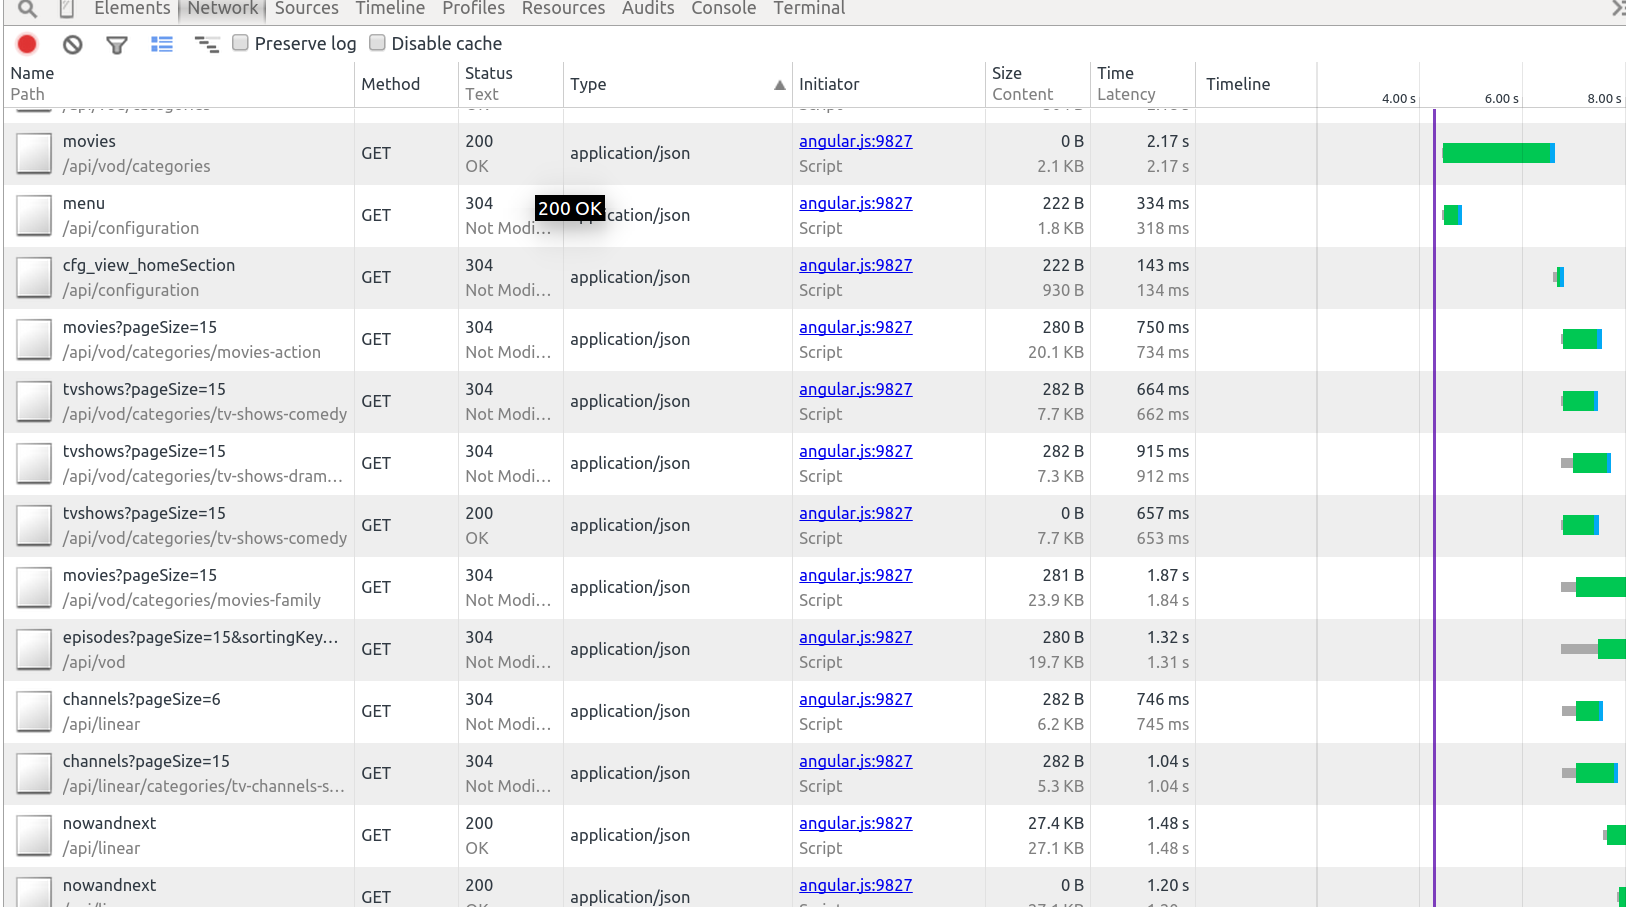
\includegraphics[width=\textwidth]{images/amount_of_requests.png}
    \caption{Example of page generation by browser}
    \label{fig:req_amount}
\end{figure}


Let’s consider system architecture using reversed proxy server instead of Redis cache. The client application will make http requests through the reversed proxy server. The proxy server will decide whether the content is stale or not and will act as a web cache. If the content is stale (non-cacheable) the proxy server will redirect the request to the middleware server. Otherwise, it will reply to the client application without touching the middleware server. The benefit of this solution is that instead of contacting server and then caching the object, the cache is contacted first and then the server. In theory, it should give the performance and flexibility. The Redis cache could be replaced by the Content Delivery Network solution in future.

% describe your solution on the top level

\subsection{Web cache selection}

The web cache for the project should satisfy several parameters:
\begin{itemize}
	\item Be Configurable- The client application sends requests both for DMOs and for writing user actions. The web cache should not cache the requests for writing user actions. The sessions still should be supported in order to write user actions. 
	\item Be Responsive, Easily Maintainable- The web cache should be deployed easily and provide statistics and internal logging. 
	\item High performance- The web cache should be transparent and must not increase the request time and latency if the cache object was not found locally. 
	% todo add more criterias
\end{itemize}

There are many web cache solutions available in both commercial and open source. For this project only open source solutions were considered. The initial candidates were: Squid, Varnish, Apache server with proxy module, Nginx server as a cachable reversed proxy, and Apache Traffic Server.

The Squid server is a forward proxy server, but it can be configured as a reversed proxy server. Squid is preferably used for storing static content.

The Varnish was developed as a reversed proxy server from the beginning. It is fast, reliable, and lightweight. It uses Varnish Configuration Language (VCL) for configuring and describing the data workflow in cache. The VCL is translated to the C code and compiled to a shared object which is then dynamically linked into the server process. It is a powerful tool that helps to set up Varnish as a dynamic reverse proxy server.

The Apache traffic server was developed by the Yahoo group and eventually moved to the Apache Incubator \cite{GuApacheTrafficUri}. According to Yahoo Inc., Apache traffic server can handle more than 400TB of internet traffic per day and works as a forward as well as reversed proxy server. It has a growing community and is continously improved upon. The configuration is simple and consists of changing several files. All these, make Apache traffic server a good candidate.  

Other solutions (Nginx and Apache server) were not originally developed to be proxy servers, but have additional modules that one can install and configure. They are not well-configured and work worse than the solutions described above \cite{GuApacheTrafficUri}[change].

A thorough comparison and performance evaluation of Varnish and Apache Traffic Server can be found in \cite{VarnApacheReverse}.    

%TODO make a benchmarking analysis of the open web proxy caches
%TODO update the report, insert thate results about benchmarking and selection

\subsection{Web cache configuration}

Before performing execution and comparative study, reversed proxy servers should be properly configured. They should aggregate and store requests that contain public data and skip analytical requests and requests with private user information (e.g. payments).

Proxy servers should also work with http sessions. Usually, when the session is specified (the set-cookie http header included in the server response), proxy servers are transparent, meaning they are skipping these requests and not storing them in memory. As was described in previous chapters, the metadata server uses http session for analytical purposes. This means that even anonymous users will have a unique session. 

In order to solve this problem, the Varnish was configured to replace Cookie header with X-Cookie header. This gives the possibility for Varnish to store the requests and still have the analytical requests available. The metadata server was modified in order to treat X-Cookie header as a Cookie header.   

\subsubsection{Varnish configuration}

The varnish logic is configured using Varnish Configurational Language(VCL). The varnish logic works as a deterministic state machine consisting of several states:

\begin{itemize}
	\item vcl\_init -- the initial state 
	\item vcl\_recv -- the initial point for the request to varnish
	\item vcl\_pass -- in this state the request is passed to the backend server
	\item vcl\_hash -- the varnish computes the hash of the request in this state
	\item vcl\_hit -- occurs when the hit is observed on varnish server
	\item vcl\_miss -- occurs when varnish has stale data or has no data at all
	\item vcl\_fetch -- when the document is acquired from the backend server
	\item vcl\_deliver -- when the cache object is about to be delivered to the client
	\item vcl\_error -- occurs when the error is observed
\end{itemize}

The Varnish configuration is presented in Appendix A.

The Varnish server starts from the command line with the appropriate arguments. The Varnish uses the following arguments:

\begin{itemize}
	\item -a : the backend server address in format ADDRESS:PORT
	\item -b : the  address in format ADDRESS:PORT
	\item -f : the path to the VCL file 
	\item -F : if specified, the varnish will be started in the foreground
	\item -n : the varnish working directory
\end{itemize} 

\subsubsection{Apache Traffic server configuration}

The Apache Traffic server configuration consists of several files: 

\begin{itemize}
	\item cache.config -- the caching behaviour is specified here
	\item remap.config  -- is used for overall configuration
	\item cluster.config -- is used for configuring Apache Traffic server in distributed mode
\end{itemize}

The Apache Traffic server uses the command line to start. The obligatory parameter is --httpport which specifies the listen port. The Apache Traffic server consists of three parts:

\begin{itemize}
	\item traffic\_cop -- supervises process for traffic\_server 
	\item traffic\_manager -- monitors the traffic\_server and gathers the logs
	\item traffic\_server -- responsible for starting the web cache server
\end{itemize}

The detailed configuration can be found \cite{ats_site}

\newpage